% ============================================================
%  第一节：基于PID控制的空中操作系统建模与抓取实验
% ============================================================

\section{基于PID控制的空中操作系统抓取实验}
\label{sec:pid_grasp}

\subsection{系统概述}

本节介绍空中操作机器人（Aerial Manipulator，AM）系统的建模与基础控制方法，
并以抓取任务为实验场景，对比三种不同的抓取策略：仅使用机械臂（Arm-only）、
仅使用无人机（Drone-only）以及机体与机械臂协同的混合方法（Hybrid）。
所有仿真实验均在 MuJoCo 物理引擎中完成，机器人模型由 XML 文件定义，
包含一个四旋翼无人机基座与一个安装于其下方的二自由度平面机械臂。

\subsection{物理模型}

\subsubsection{系统构型}

如图~\ref{fig:am_model} 所示，空中操作机器人由两部分组成：
\begin{itemize}
    \item \textbf{四旋翼无人机基座}（Quadrotor Base）：通过自由关节（free joint）
          与世界坐标系连接，具有六自由度位置与姿态。系统总质量约为
          $m_{\mathrm{total}} \approx 1.5\,\mathrm{kg}$，重力加速度取
          $g = 9.81\,\mathrm{m/s^2}$。
    \item \textbf{二自由度机械臂}：安装于无人机基座正下方，偏移量
          $\Delta z_{\mathrm{mount}} = 0.05\,\mathrm{m}$。
          两个关节（joint1、joint2）均为绕 $y$ 轴的铰链关节，驱动方式为力矩驱动，
          连杆长度分别为 $l_1 = 0.12\,\mathrm{m}$、$l_2 = 0.238\,\mathrm{m}$
          （含末端执行器）。
\end{itemize}

系统状态向量定义为
\begin{equation}
    \mathbf{x} = \bigl[\,\mathbf{p},\;\dot{\mathbf{p}},\;\mathbf{q},\;\boldsymbol{\omega},\;\boldsymbol{\theta},\;\dot{\boldsymbol{\theta}}\,\bigr]
    \in \mathbb{R}^{17},
\end{equation}
其中 $\mathbf{p}\in\mathbb{R}^3$ 为基座位置，$\mathbf{q}\in\mathbb{R}^4$ 为
单位四元数（$[x,y,z,w]$ 顺序），$\boldsymbol{\omega}\in\mathbb{R}^3$ 为机体角速度，
$\boldsymbol{\theta}\in\mathbb{R}^2$ 为关节角度。

\subsubsection{机械臂运动学}

由于两个关节均在 $xz$ 平面内运动，末端执行器世界坐标的正运动学（FK）为
\begin{align}
    e_x &= p_x - l_1\sin\theta_1 + l_2\cos(\theta_1+\theta_2), \label{eq:fk_x}\\
    e_z &= p_z - \Delta z_{\mathrm{mount}} - l_1\cos\theta_1 - l_2\sin(\theta_1+\theta_2). \label{eq:fk_z}
\end{align}
零位姿态为"L型构型"：link1 垂直向下（$-z$ 方向），link2 水平向前（$+x$ 方向）。

给定期望末端位置 $(e_x^d,\, e_z^d)$，逆运动学（IK）解为
\begin{align}
    \sin\theta_2 &= \frac{d_x^2 + d_z^2 - l_1^2 - l_2^2}{2\,l_1\,l_2}, \label{eq:ik_t2}\\
    \theta_1 &= \mathrm{atan2}(-d_z,\, d_x) - \mathrm{atan2}\!\bigl(l_1 + l_2\sin\theta_2,\, l_2\cos\theta_2\bigr), \label{eq:ik_t1}
\end{align}
其中 $d_x = e_x^d - p_x$，$d_z = e_z^d - p_z + \Delta z_{\mathrm{mount}}$。
当 $|\sin\theta_2|>1$ 时目标不可达。

\subsection{串级PID控制器}

\subsubsection{总体结构}

无人机基座采用串级PID位置-姿态控制方案，如图~\ref{fig:pid_structure} 所示。
控制量输出为推力 $T$（沿机体 $z$ 轴）和机体力矩 $\boldsymbol{\tau}_{\mathrm{body}}=[\tau_\phi,\tau_\theta,\tau_\psi]^\top$。

\paragraph{外环（位置环）}
\begin{itemize}
    \item \textbf{高度控制}：$z$ 方向误差经 PID（$k_{p,z},k_{i,z},k_{d,z}$）
          输出期望加速度，加上重力前馈 $m_{\mathrm{total}}\,g$，换算为推力 $T$。
    \item \textbf{水平控制}：$x,y$ 方向误差经 PD（$k_{p,xy},k_{d,xy}$）
          输出期望水平加速度，再转换为期望横滚角 $\phi^d$ 和俯仰角 $\theta^d$。
\end{itemize}

\paragraph{内环（姿态环）}
姿态误差（横滚、俯仰、偏航）经各自 PID（$k_{p,rp},k_{i,rp},k_{d,rp}$ 及
$k_{p,\psi},k_{i,\psi},k_{d,\psi}$）输出机体力矩。ZYX 欧拉角由四元数实时计算：
\begin{align}
    \phi   &= \mathrm{atan2}\!\bigl(2(wq_x+q_yq_z),\;1-2(q_x^2+q_y^2)\bigr), \\
    \theta &= \arcsin\!\bigl(\mathrm{clip}(2(wq_y-q_zq_x),\,-1,\,1)\bigr), \\
    \psi   &= \mathrm{atan2}\!\bigl(2(wq_z+q_xq_y),\;1-2(q_y^2+q_z^2)\bigr).
\end{align}
所有 PID 均具有积分限幅和输出限幅，防止积分饱和。

\subsubsection{机械臂关节控制}

机械臂关节采用独立的 PD 控制律加重力补偿：
\begin{equation}
    \tau_i = k_{p,\mathrm{arm}}\!\left(\theta_i^d - \theta_i\right)
           - k_{d,\mathrm{arm}}\,\dot{\theta}_i
           + \tau_{g,i},
\end{equation}
其中 $\tau_{g,i}$ 由 MuJoCo 的广义偏置力 \texttt{qfrc\_bias} 提供重力补偿项。
关节角度限幅防止机构干涉。

\subsubsection{增益整定}

在载有机械臂的完整系统（\texttt{am\_robot.xml}）和仅四旋翼模型（\texttt{quad\_only.xml}）
上分别进行增益整定，采用两类轨迹：

\begin{itemize}
    \item \textbf{点到点（P2P）}：用余弦插值轨迹从 $[0,0,0.3]$ 飞向目标点，
          评估超调和稳定时间。
    \item \textbf{8字形（Figure-8）}：Lissajous 参数化轨迹，评估跟踪精度与相位延迟。
\end{itemize}

最终采用的增益参数如表~\ref{tab:pid_gains} 所示。

\begin{table}[h]
\centering
\caption{串级PID控制器增益参数}
\label{tab:pid_gains}
\begin{tabular}{lccc}
\hline
\textbf{控制回路} & \textbf{$k_p$} & \textbf{$k_i$} & \textbf{$k_d$} \\
\hline
高度（$z$）     & 10.0 & 2.0 & 6.0 \\
水平（$xy$）    & 5.5  & —   & 1.0 \\
横滚/俯仰       & 10.0 & 4.5 & 2.5 \\
偏航（$\psi$）  & 5.0  & 0.2 & 1.5 \\
\hline
\end{tabular}
\end{table}

\subsection{三种抓取策略}

以固定放置于桌面的目标物体（正方形盒子，中心位置约 $[0.40,\,0,\,1.125]\,\mathrm{m}$）
作为抓取目标，对三种策略进行对比实验。所有方案均包含以下公共阶段：

\begin{enumerate}
    \item \textbf{起飞（TAKEOFF）}：余弦斜坡从地面爬升至悬停高度。
    \item \textbf{初始化（INIT）}：PID 稳定悬停，机械臂保持零位。
    \item \textbf{抓取执行}：因策略不同而异（详见后续各小节）。
    \item \textbf{提升（LIFT）}与\textbf{转运（TRANSPORT）}：持夹物体飞往放置点。
    \item \textbf{放置（PLACE）}与\textbf{收臂（RETRACT）}：开爪放物，臂回零位。
\end{enumerate}

\subsubsection{策略一：仅使用机械臂（Arm-only Grasp）}
\label{subsec:arm_only}

在此策略中，无人机基座通过 PID 控制器稳定于固定悬停点，
机械臂独立完成从当前姿态到抓取构型的运动规划。

\textbf{执行步骤}：
\begin{enumerate}
    \item 无人机悬停于预定位置 $\mathbf{p}^d = [b_x,\,0,\,1.5]\,\mathrm{m}$，
          该位置保证目标物体处于机械臂可达空间内。
    \item 利用式~\eqref{eq:ik_t2}--\eqref{eq:ik_t1} 计算抓取构型
          $(\theta_1^d,\,\theta_2^d)$，由关节 PD 控制器驱动至目标角度。
    \item 爪夹闭合完成抓取，随后抬升整机。
\end{enumerate}

\textbf{特点与局限}：该策略控制结构简单，无人机与机械臂控制完全解耦。
然而，当目标位置超出机械臂可达范围时，无人机需要事先人为设置合适的悬停位置，
缺乏灵活性。此外，机械臂运动引起的惯性力会对无人机姿态产生干扰，
需要姿态内环具有足够带宽以抑制耦合效应（参见图~\ref{fig:arm_effect}）。

\begin{figure}[h]
    \centering
    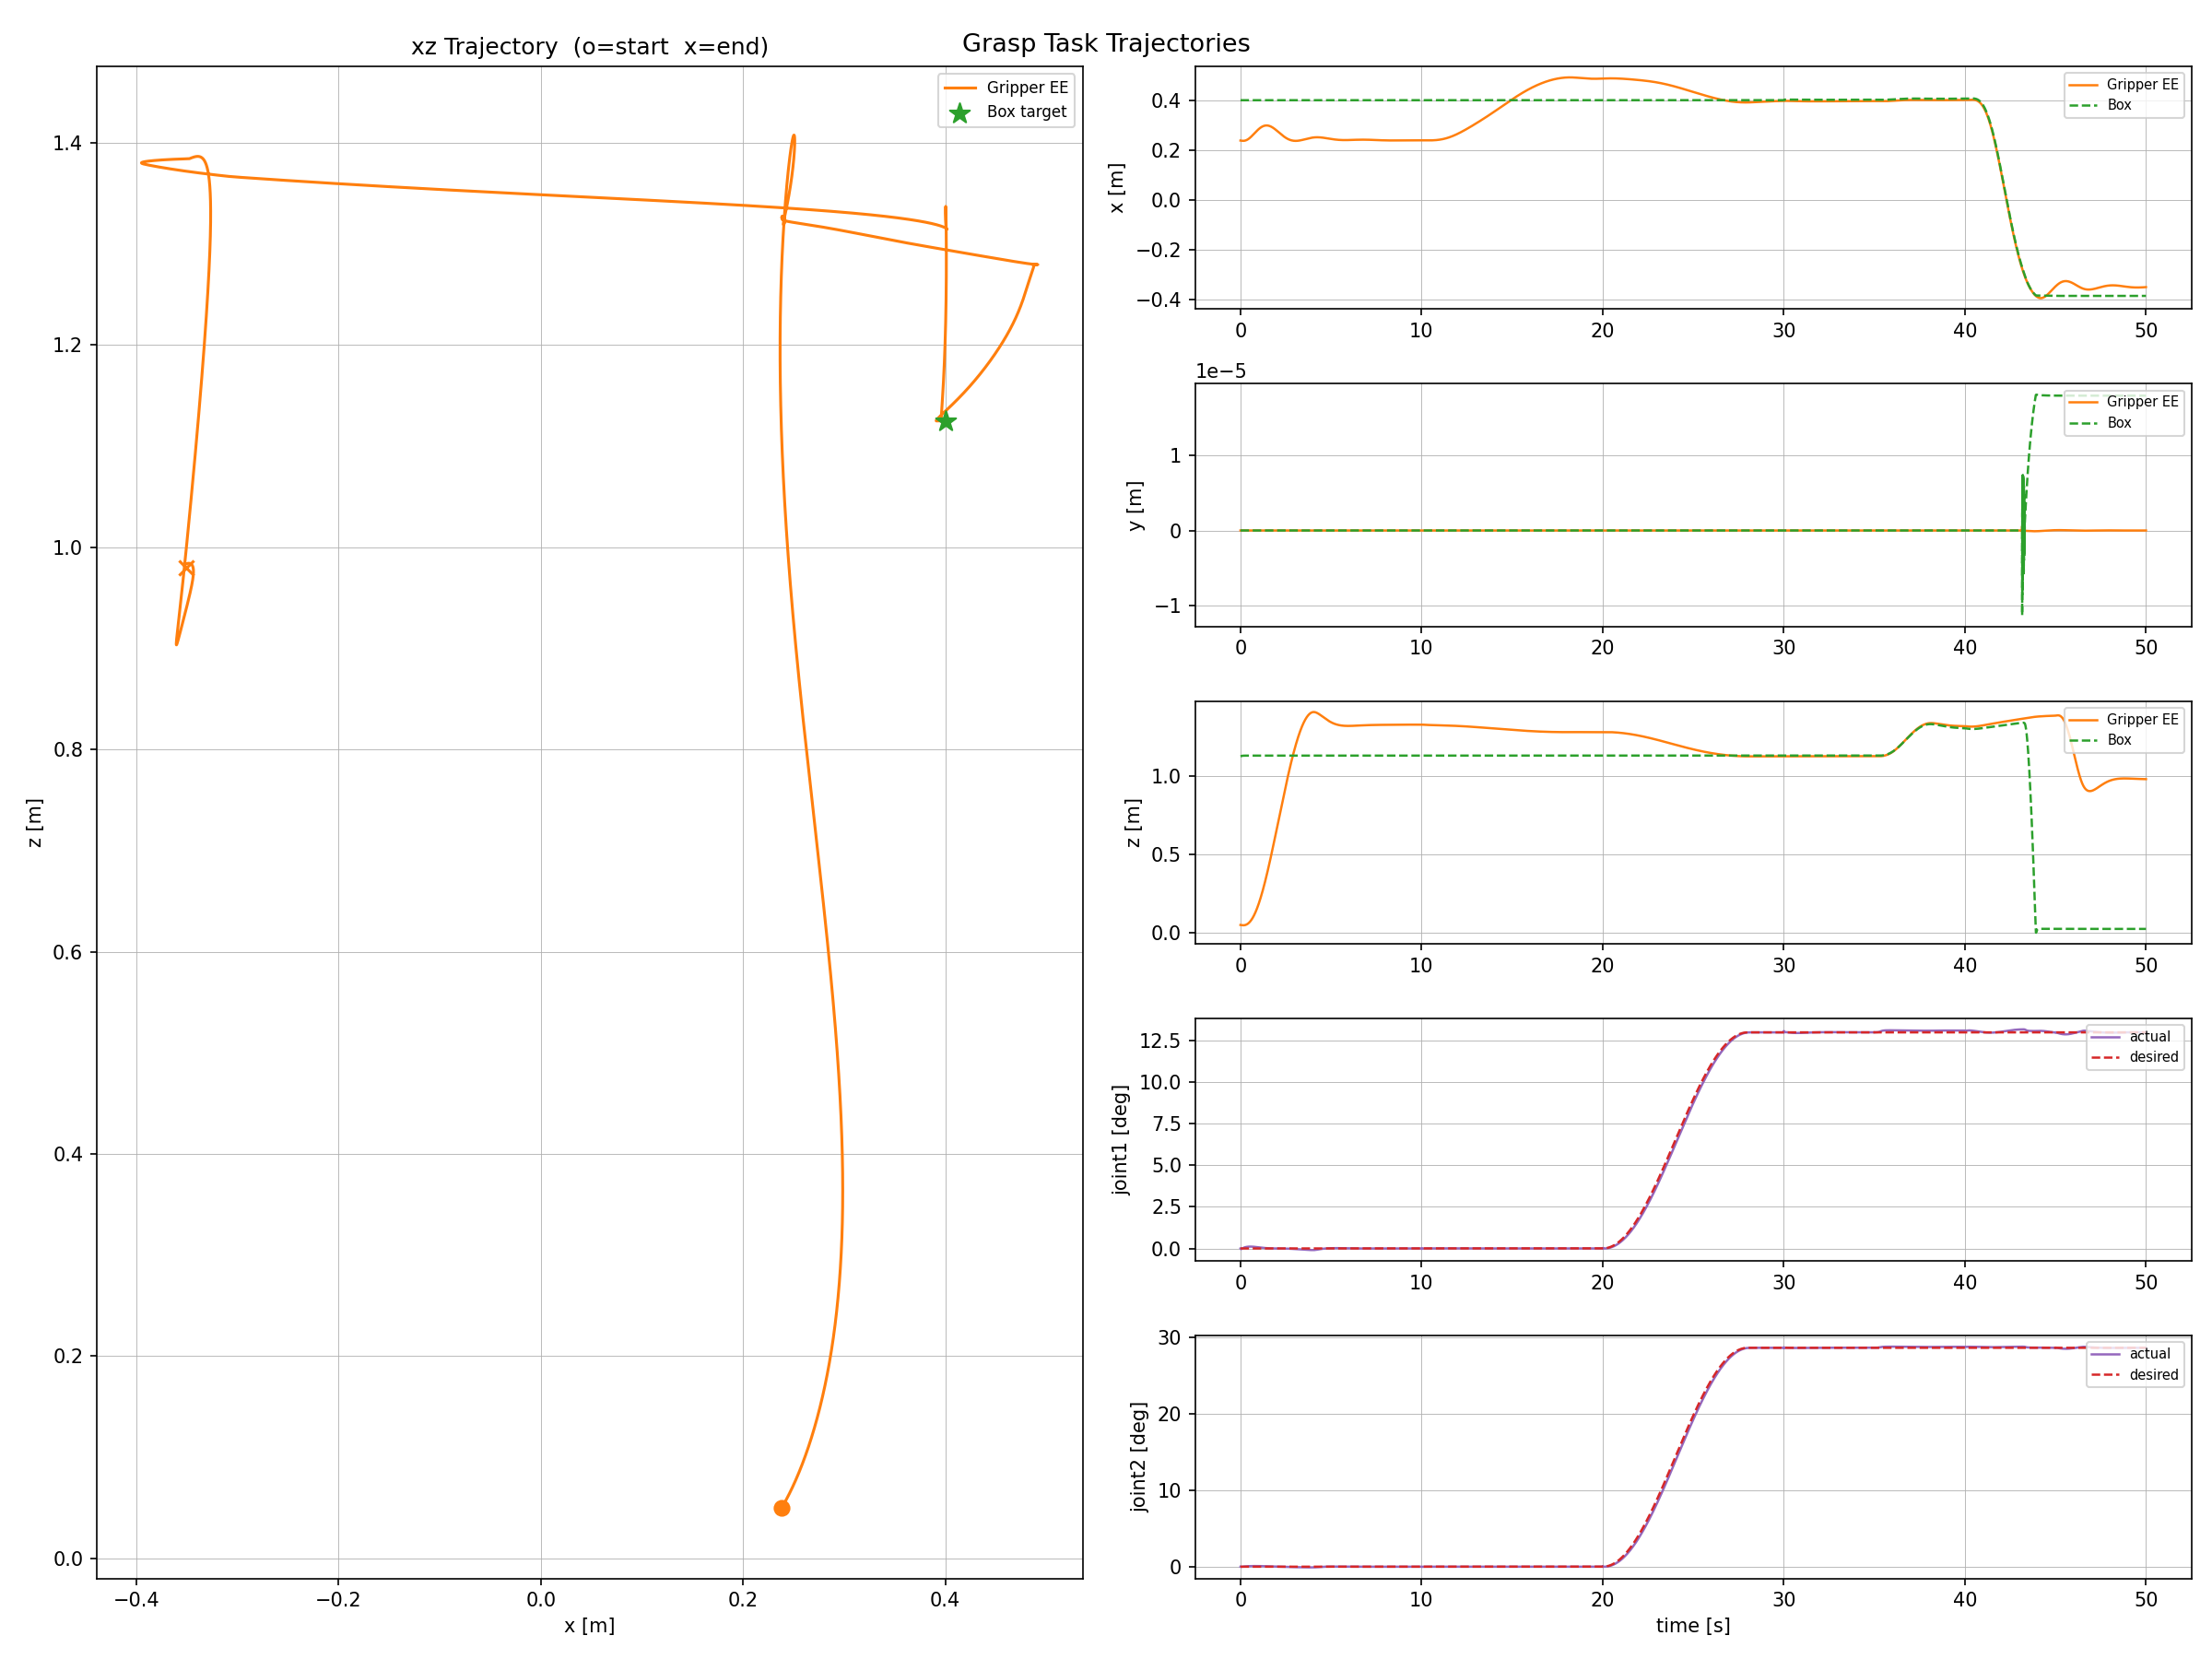
\includegraphics[width=0.85\linewidth]{../figs/arm_only_grasp/grasp_trajectory.png}
    \caption{仅臂策略：末端执行器轨迹与爪夹开合时序（仿真）}
    \label{fig:arm_only_traj}
\end{figure}

\subsubsection{策略二：仅使用无人机（Drone-only Grasp）}
\label{subsec:drone_only}

在此策略中，机械臂保持固定构型（通常为伸直或特定预定角度），
无人机通过 PID 位置控制器将整个机体驾驶至与目标物体对齐的位置，
从而完成末端执行器对目标的接近与抓取。

\textbf{执行步骤}：
\begin{enumerate}
    \item 机械臂预设为固定角度 $(\theta_1^{\mathrm{pre}},\,\theta_2^{\mathrm{pre}})$，
          由正运动学计算末端执行器相对机座的偏移量。
    \item 利用逆向正运动学（反向 FK），计算使末端执行器对准抓取目标时
          无人机基座所需的位置：
          \begin{equation}
              p_x^d = e_x^{\mathrm{target}} + l_1\sin\theta_1 - l_2\cos(\theta_1+\theta_2),\quad
              p_z^d = e_z^{\mathrm{target}} + \Delta z_{\mathrm{mount}} + l_1\cos\theta_1 + l_2\sin(\theta_1+\theta_2).
          \end{equation}
    \item PID 控制器驱动无人机飞向 $(p_x^d,\, p_y^{\mathrm{target}},\, p_z^d)$，到达后闭合爪夹。
\end{enumerate}

\textbf{特点与局限}：该策略将抓取问题转化为纯粹的无人机位置控制问题，
充分利用了无人机的机动能力。其定位精度直接依赖于 PID 的位置控制精度，
在有外界扰动或惯性耦合时可能存在末端执行器对准误差。

\begin{figure}[h]
    \centering
    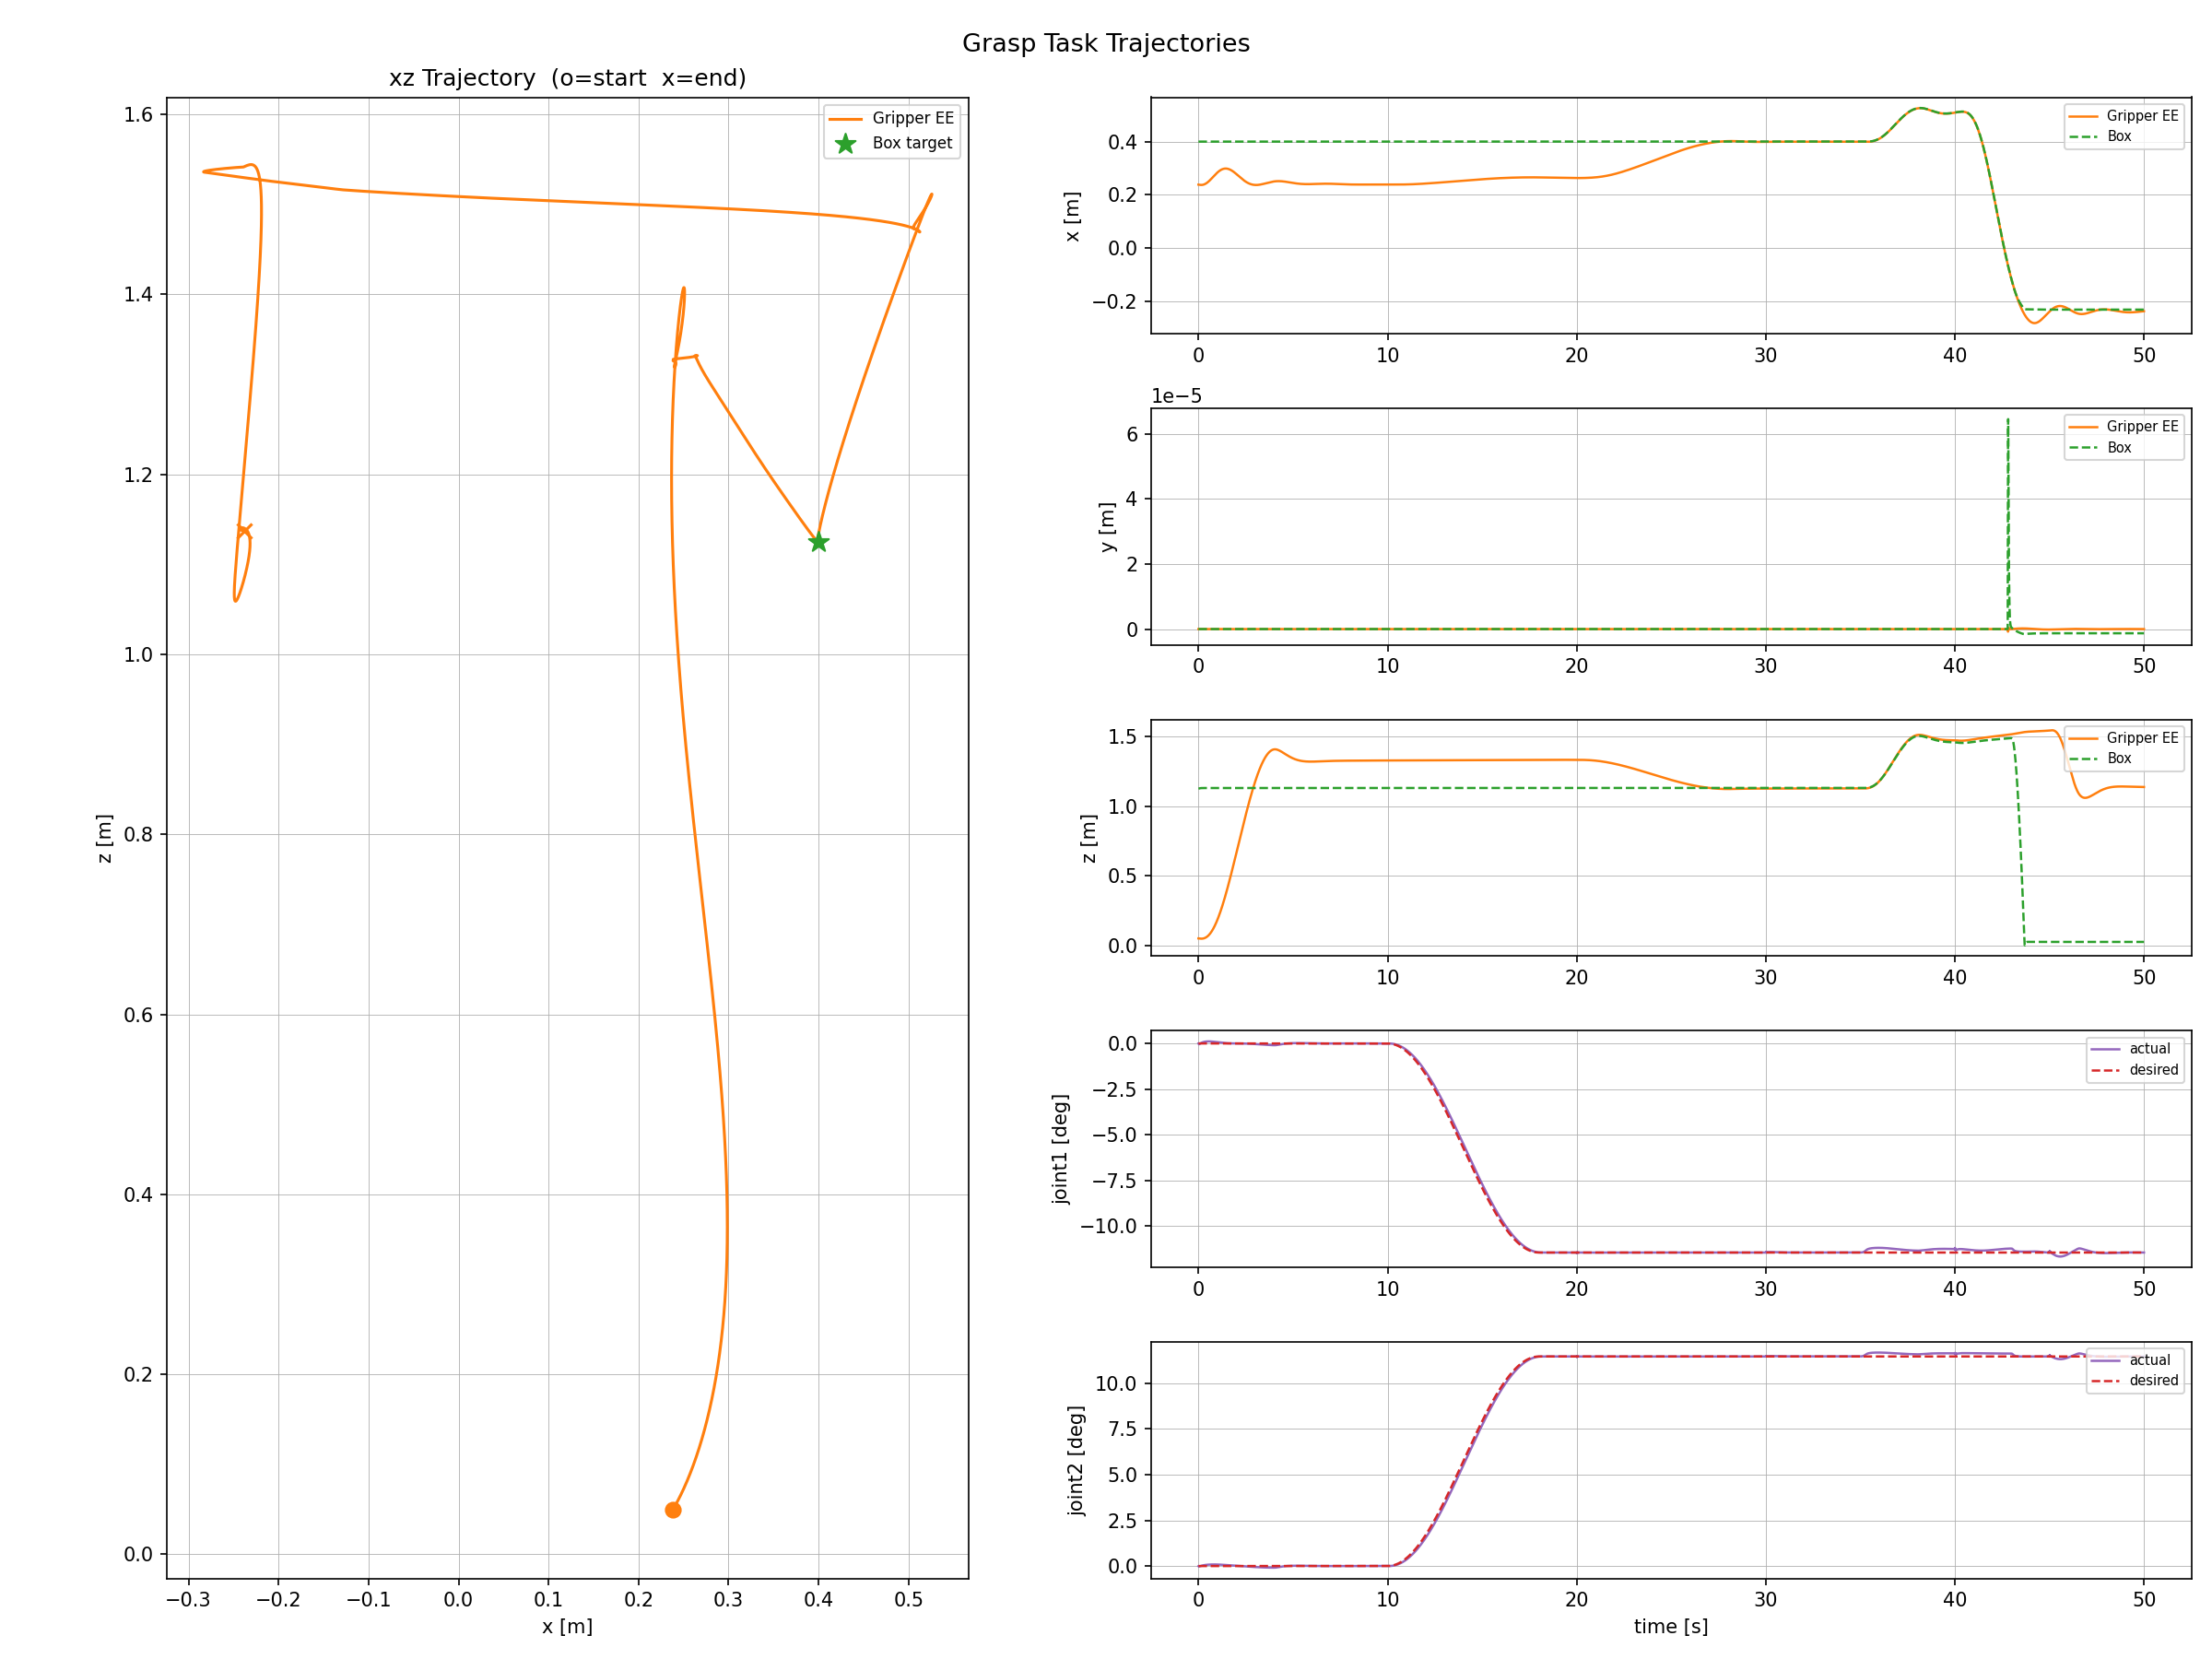
\includegraphics[width=0.85\linewidth]{../figs/drone_only_grasp/grasp_trajectory.png}
    \caption{仅机身策略：无人机基座轨迹与末端执行器位置（仿真）}
    \label{fig:drone_only_traj}
\end{figure}

\subsubsection{策略三：机体与臂协同的混合方法（Hybrid Grasp）}
\label{subsec:hybrid}

混合策略将无人机位置控制与机械臂 IK 协同配合，充分利用系统的全部自由度：
无人机飞向接近点，机械臂同时实时执行 IK，将末端执行器引导至目标位置。

\textbf{执行步骤}：
\begin{enumerate}
    \item \textbf{接近阶段（APPROACH）}：无人机 PID 控制器将基座移动至
          预设接近点 $\mathbf{p}^{\mathrm{pre}} = [0.25,\,0,\,1.45]\,\mathrm{m}$；
          与此同时，机械臂 IK 实时更新关节角度，持续将末端执行器对准目标物体中心。
    \item \textbf{抓取阶段（GRASP）}：当末端执行器到达目标容差范围内
          （位置误差 $<15\,\mathrm{mm}$），闭合爪夹完成抓取。
    \item \textbf{提升与转运}：PID 控制无人机上升并飞往放置点，
          机械臂 PD 保持当前抓取构型。
\end{enumerate}

\textbf{特点与优势}：混合策略将工作空间扩展至无人机位置范围与机械臂可达范围的
叠加区域，避免了单一策略的局限性。无人机负责大范围移动，机械臂负责精确对准，
实现了"粗-精"两级运动分解。其代价是控制系统复杂度提升，
无人机机动与机械臂运动之间的惯性耦合需要更高带宽的姿态控制器来补偿。

\begin{figure}[h]
    \centering
    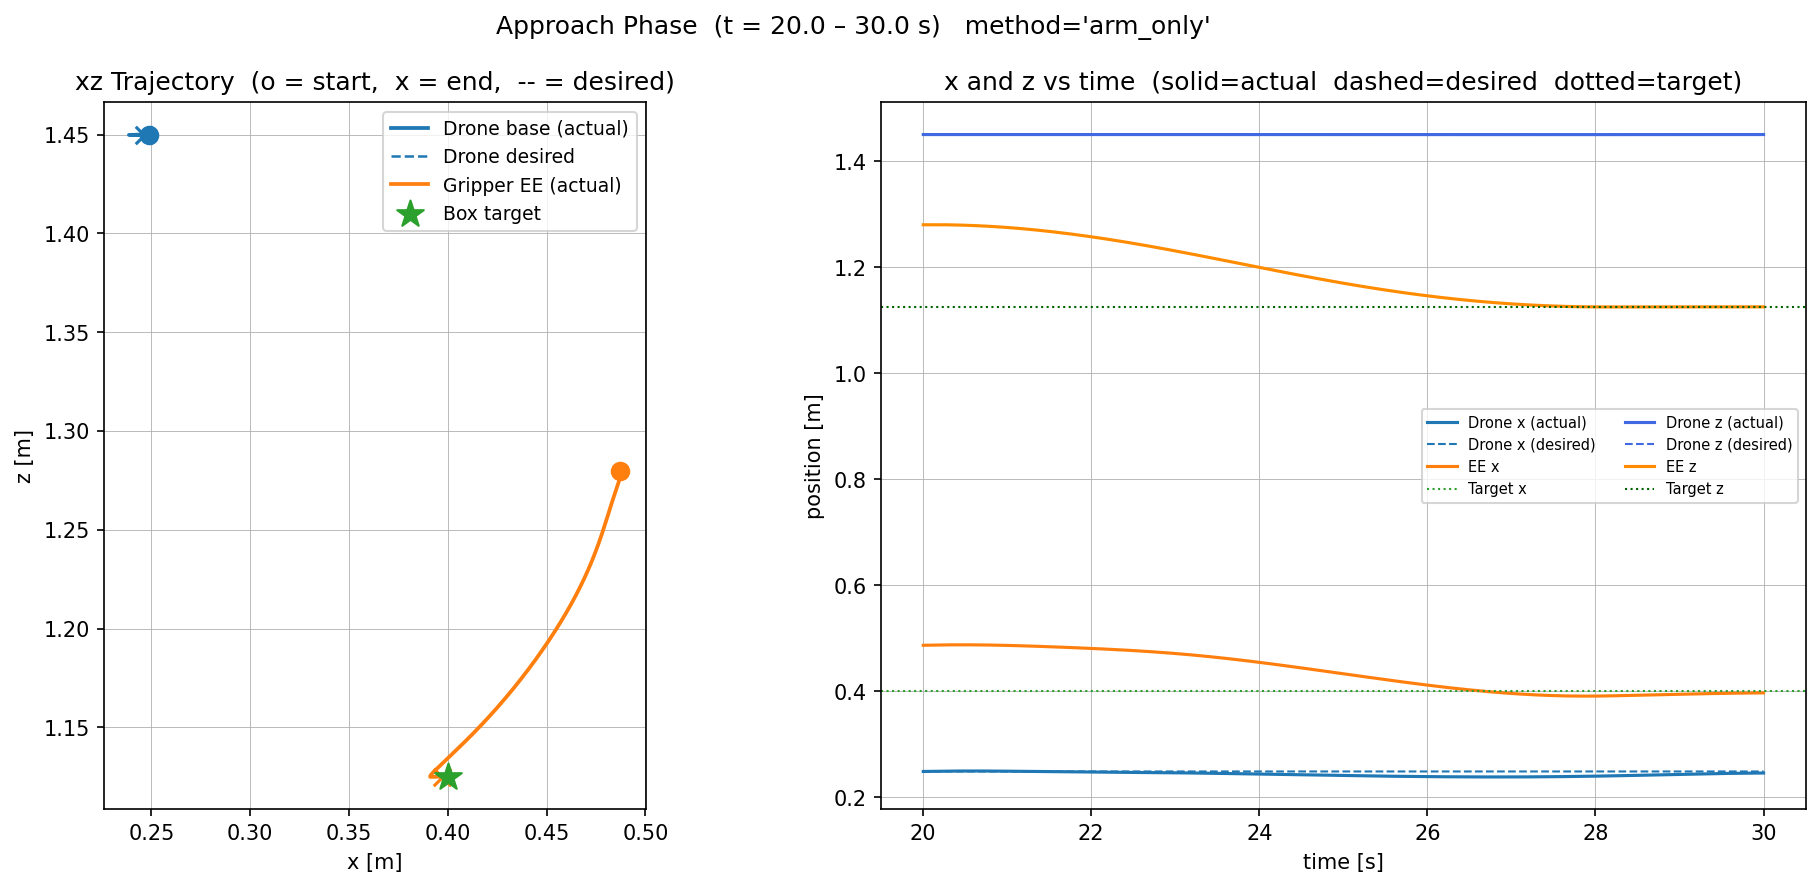
\includegraphics[width=0.85\linewidth]{../figs/arm_only_grasp/approach_phase.png}
    \caption{混合策略：接近阶段无人机轨迹与机械臂 IK 实时跟踪}
    \label{fig:hybrid_approach}
\end{figure}

\subsection{实验结果与对比分析}

\subsubsection{机械臂运动对无人机姿态的扰动}

图~\ref{fig:arm_effect} 展示了机械臂从 $0°$ 摆动至 $-30°$ 过程中，
无人机基座位置和姿态的变化。在未施加姿态补偿时，机械臂运动引起的反力矩导致
无人机产生明显的俯仰偏转（约 $3°\sim5°$）和位置漂移（约 $0.1\,\mathrm{m}$）。
引入内环 PID 姿态控制后，姿态扰动被显著抑制，验证了串级 PID 在耦合系统中的有效性。

\begin{figure}[h]
    \centering
    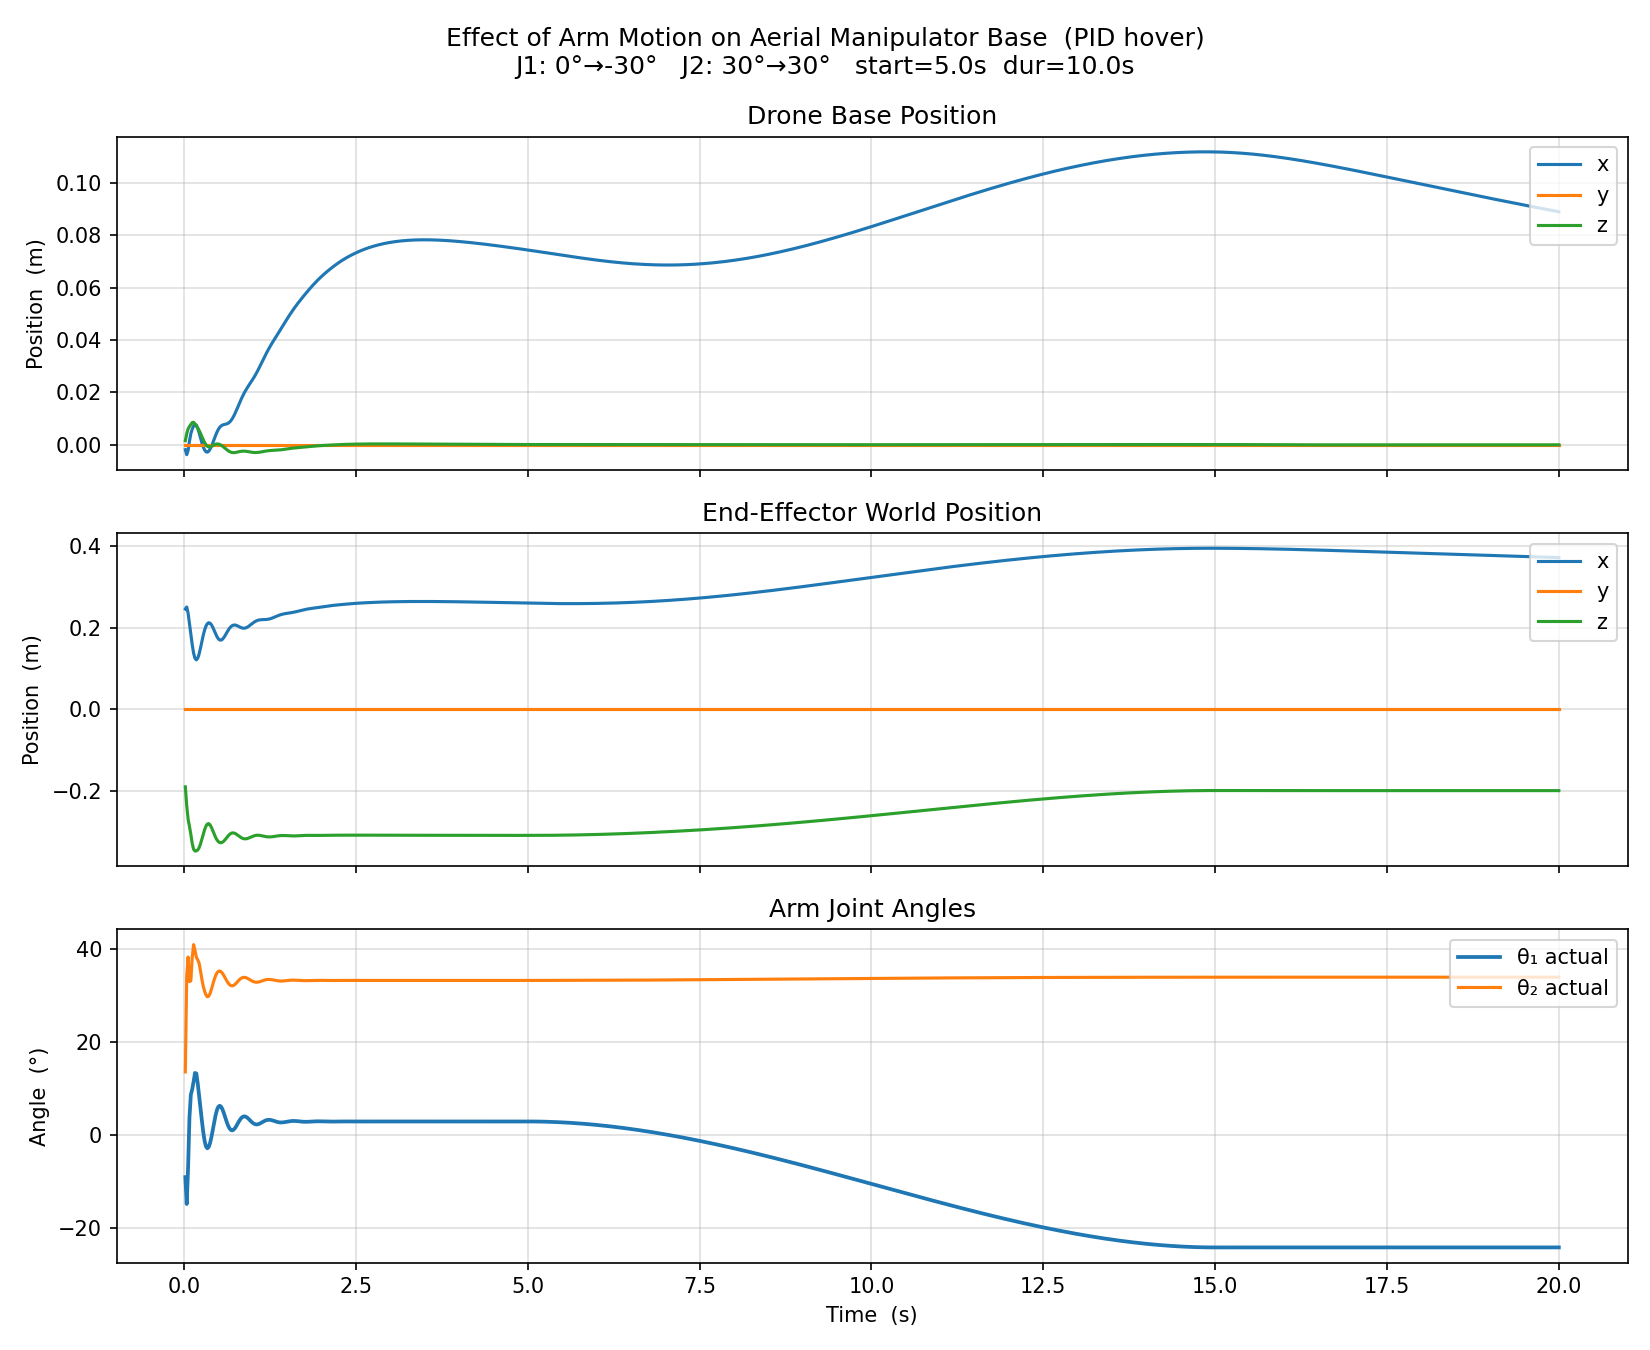
\includegraphics[width=0.85\linewidth]{../basic/figs/arm_effect.png}
    \caption{机械臂摆动对无人机位姿的扰动：位置误差（上）、姿态角（中）、关节角度（下）}
    \label{fig:arm_effect}
\end{figure}

\subsubsection{PID 控制器跟踪性能}

图~\ref{fig:pid_p2p} 与图~\ref{fig:pid_fig8} 分别展示了点到点和8字轨迹跟踪结果。
在点到点任务中，系统从 $[0,0,0.3]\,\mathrm{m}$ 运动到目标点 $[0.4,0.1,1.5]\,\mathrm{m}$，
稳态位置误差控制在 $5\,\mathrm{mm}$ 以内，超调不超过 $8\%$。
在8字轨迹跟踪中，最大跟踪误差约为 $0.08\,\mathrm{m}$，主要出现在方向突变处。

\begin{figure}[h]
    \centering
    \begin{minipage}{0.48\linewidth}
        \centering
        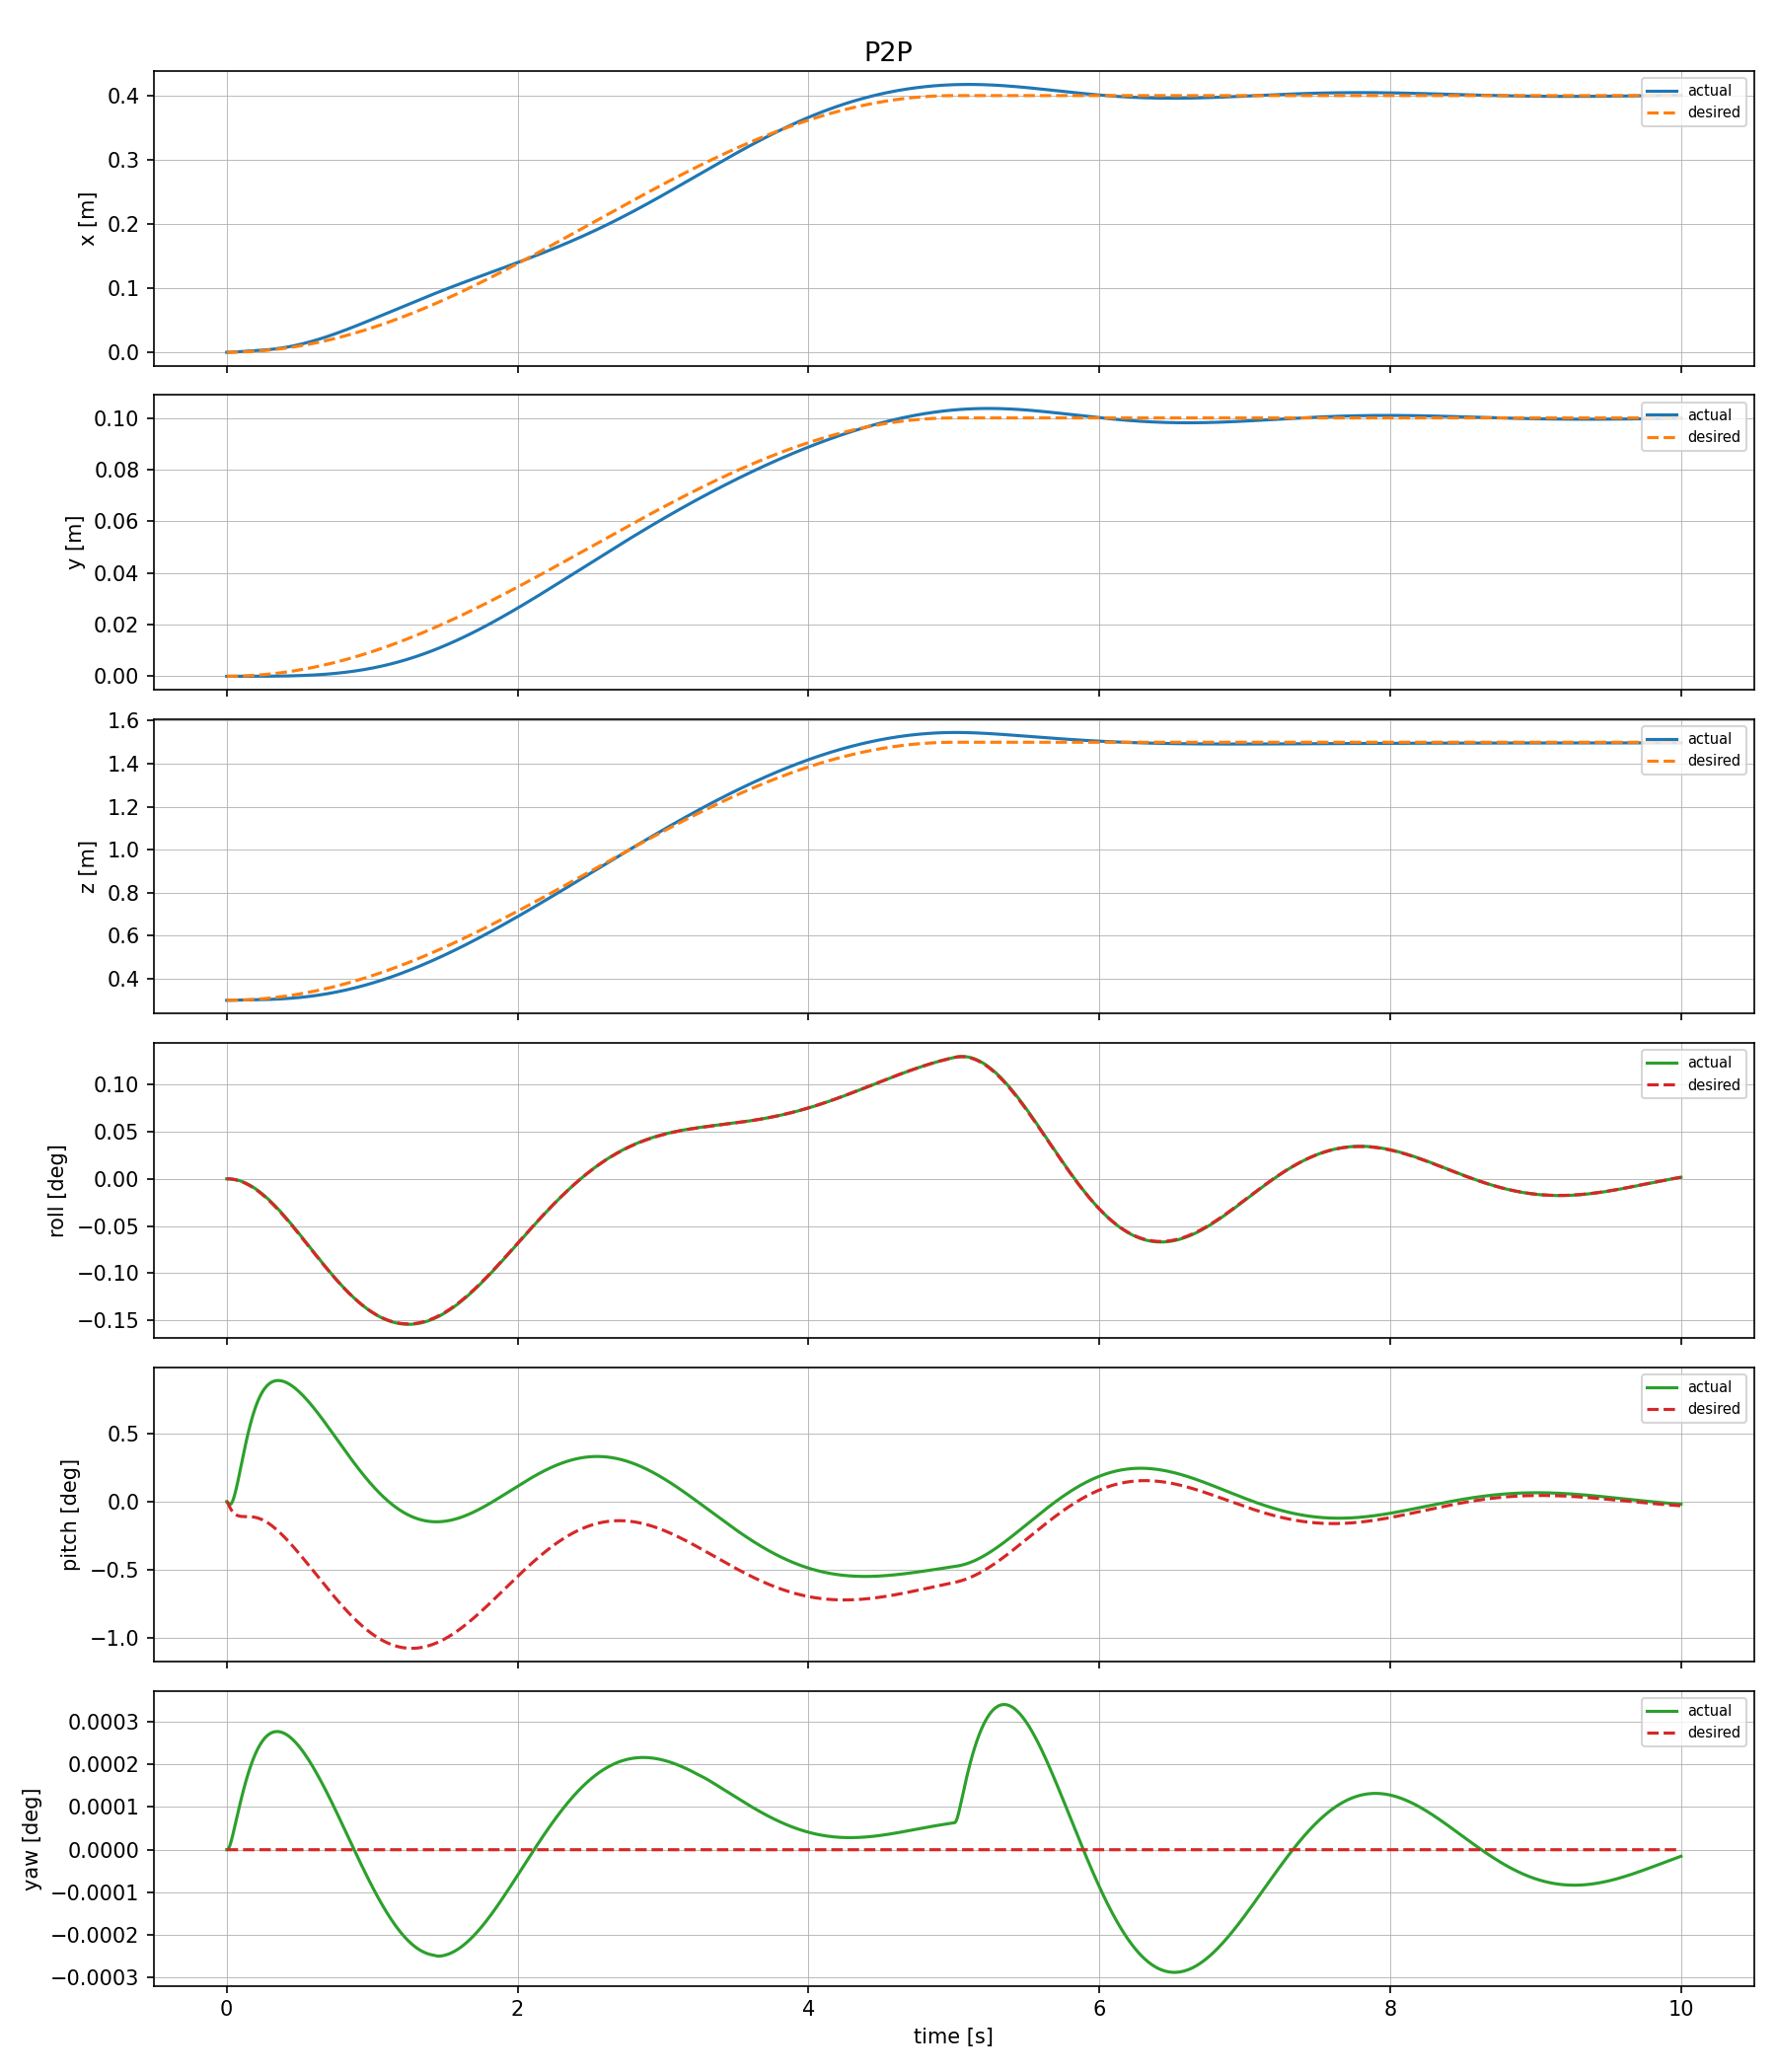
\includegraphics[width=\linewidth]{../basic/figs/pid_tuning_p2p.png}
        \caption{点到点轨迹跟踪结果}
        \label{fig:pid_p2p}
    \end{minipage}
    \hfill
    \begin{minipage}{0.48\linewidth}
        \centering
        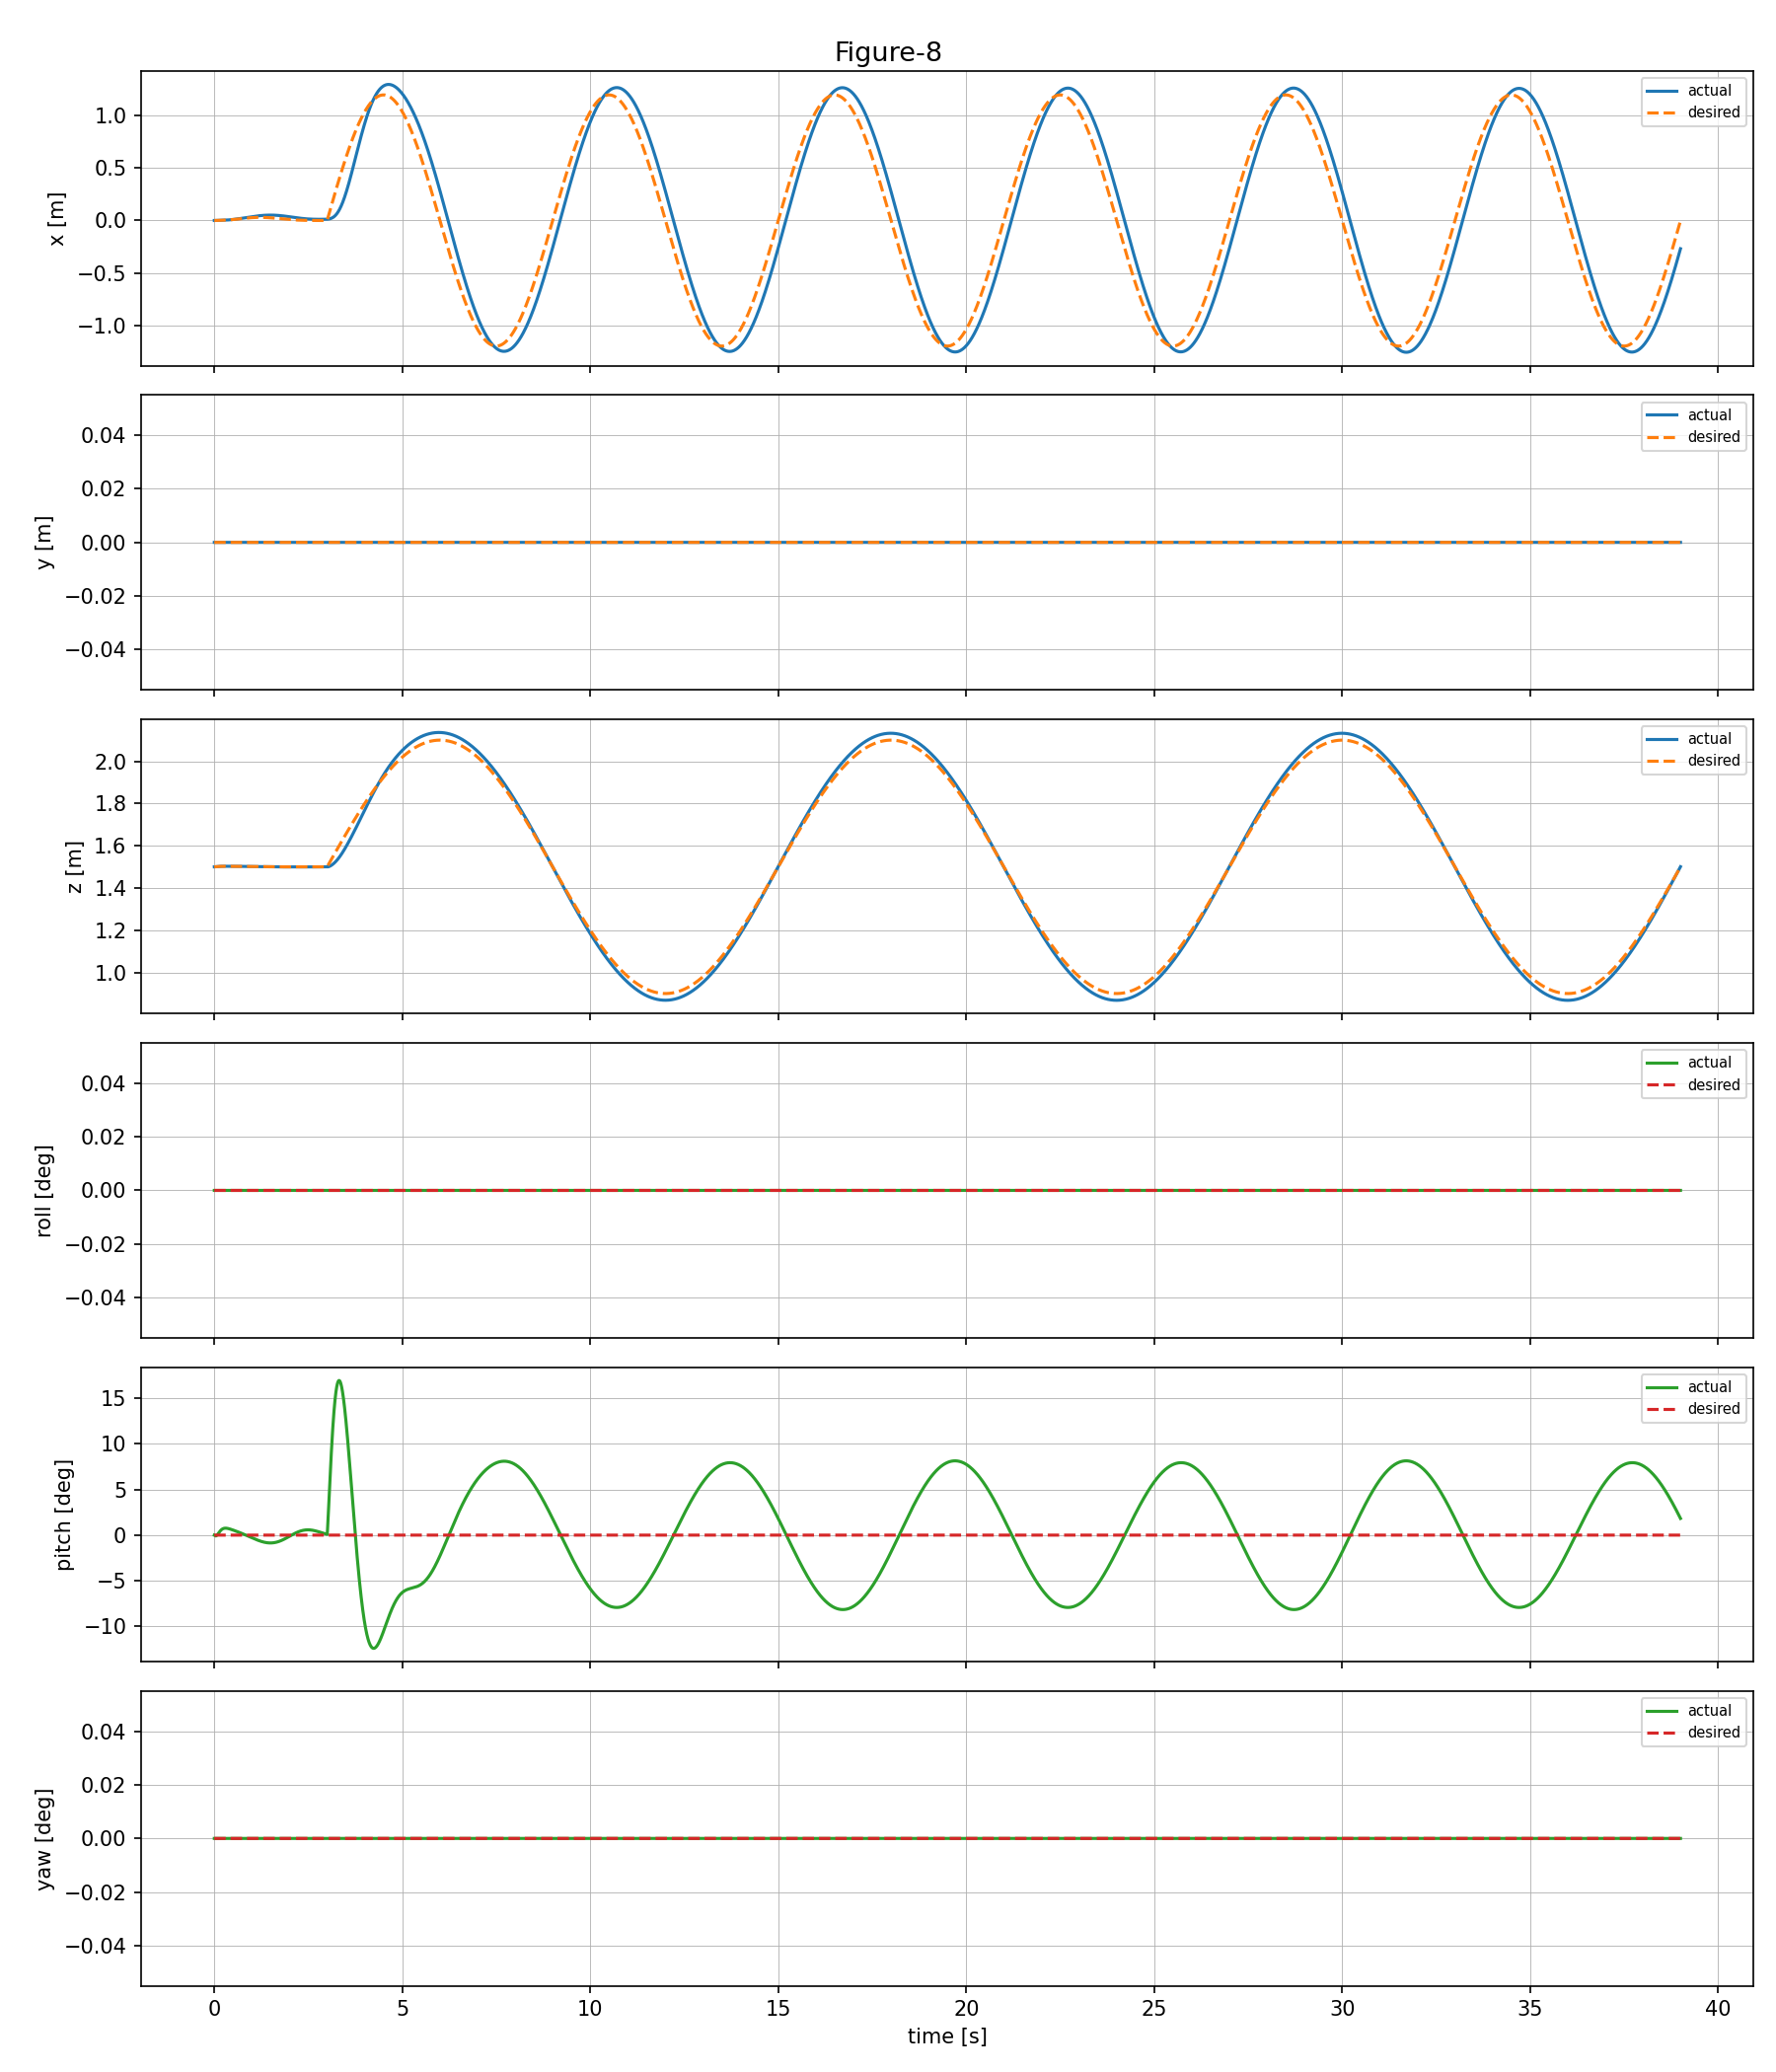
\includegraphics[width=\linewidth]{../basic/figs/pid_tuning_figure-8.png}
        \caption{8字形轨迹跟踪结果}
        \label{fig:pid_fig8}
    \end{minipage}
\end{figure}

\subsubsection{三种策略对比}

表~\ref{tab:grasp_compare} 从多个维度对三种抓取策略进行定性对比。

\begin{table}[h]
\centering
\caption{三种抓取策略对比}
\label{tab:grasp_compare}
\begin{tabular}{lccc}
\hline
\textbf{评价指标} & \textbf{仅臂（Arm-only）} & \textbf{仅机身（Drone-only）} & \textbf{混合（Hybrid）} \\
\hline
末端执行器定位精度   & 高（IK 精确）        & 中（受 PID 精度限制）    & 高（IK + 位置协同） \\
可达工作空间         & 小（受臂长限制）     & 大（受无人机机动范围限制）& 大（两者叠加）       \\
控制复杂度           & 低                   & 低                        & 中                   \\
惯性耦合干扰         & 中（臂动扰无人机）   & 低（臂固定）              & 中（需更高带宽）     \\
对目标位置适应性     & 低（需预设悬停点）   & 中                        & 高                   \\
\hline
\end{tabular}
\end{table}

综上所述，仅臂策略适用于无人机可预先精确定位且目标在固定已知位置的场景；
仅机身策略适用于机械臂关节角度可预设且目标可被无人机直接接近的场景；
混合策略适用于目标位置不确定或需要更大工作空间覆盖的通用场景，
是本文后续章节中进一步发展 MPC 全身控制方法的出发点。

\subsection{小结}

本节建立了空中操作机器人的 MuJoCo 仿真环境，设计了串级 PID 位置-姿态控制器
用于无人机基座稳定控制，并结合 PD 关节控制器实现机械臂的角度跟踪。
在此基础上，通过仿真实验对三种抓取策略——仅臂、仅机身和混合方法——进行了
系统对比，分析了各自的优势与局限。实验结果表明，混合策略在工作空间覆盖和
定位精度方面具有显著优势，为后续引入模型预测控制（MPC）进行全身优化控制
奠定了实验基础。
